\documentclass{beamer}
\usetheme[colour=UoEblue]{UsherNew}
%% Alternative options are:
%\usetheme[colour=USHERgreen]{UsherNew}
%\usetheme[colour=USHERblue]{UsherNew}
\usepackage{beamernotes}
\usepackage{amsmath}
\pdfcompresslevel=9
\pdfobjcompresslevel=3

\title[]{Decrypting Elliptic Curves...}
\subtitle{Decrypting Elliptic Curves...}
\author{Benjamin Brown}
%\institute{Institute Name}
\date{3\textsuperscript{rd} July 2020}

\begin{document}

\begin{frame}
  \titlepage
\end{frame}
\bnote{This generates notes for pdfpc. These notes also appear
  on the handout/article versions.}

\begin{frame}[t]{Ellipses}
	After circles, ellipses are the most familiar curves in mathematics.
	\begin{figure}[h]
		\centering
		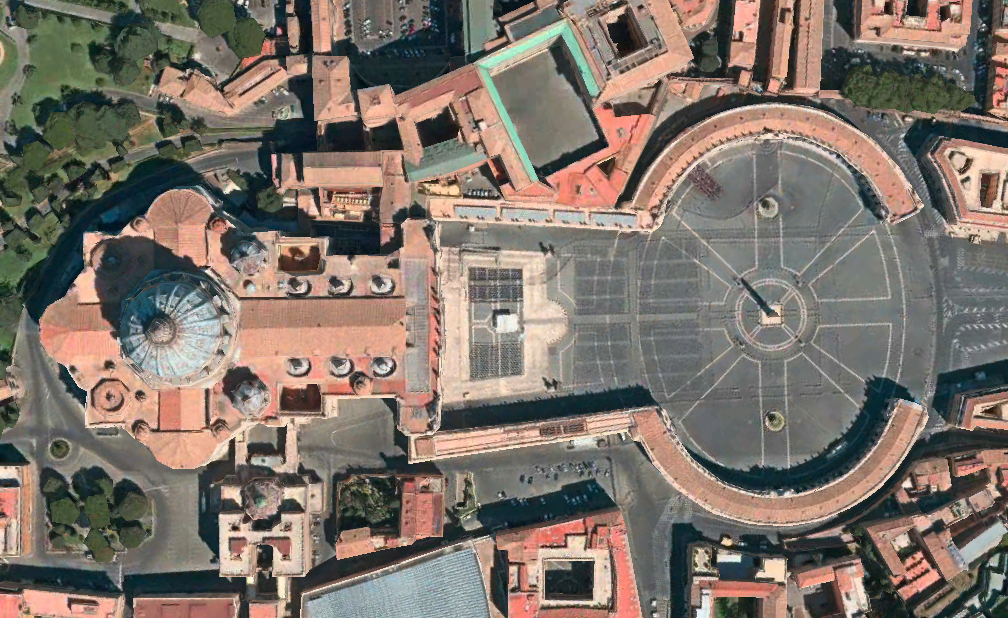
\includegraphics[width=10cm]{st-patricks-square}
		\caption{St Patrick's Square.}
	\end{figure}
\end{frame}

\begin{frame}	
	copy page over
\end{frame}

\begin{frame}[t]{Elliptic Functions}
	Arc-length of an ellipse?
\begin{equation*}
	x = a\cos\theta,\quad y=b\sin\theta\quad \quad \quad 
\end{equation*}
	
\begin{equation*}
	\begin{split}
		L &= \int_{0}^{2\pi} \sqrt{ ( \partial_{\theta}x )^{2} + ( \partial_{\theta}y )^{2} }\, d\theta \\
		&= 4a \int_{0}^{1} \sqrt{ 1 - k^{2} u^{2} }\, du \quad (k^{2} = (a^{2} - b^{2})/a^{2};\quad u = \sin\theta ) \\
		&= \frac{1}{2} \int_{1-k^{2}}^{1} \frac{t\, dt}{\sqrt{t(t-1)(t - (1-k^{2}))}}\quad (t = 1 - k^{2}u^{2})
	\end{split}
\end{equation*}	
\end{frame}

\begin{frame}
	Integrals of the form
	\begin{equation*}
		w = f(z) = \int_{P}^{z} \frac{t\, dt}{c_{3}t^{3} + c_{2}t^{2} + c_{1}t + c_{0}}
	\end{equation*}
	are called \emph{elliptic integrals (of the 2\textsuperscript{nd} kind)}. \\~\\
	
	In general, involve integrals with square-roots of cubic or quartic polynomials. \\~\\
	
	\emph{Elliptic functions} are the inverses to elliptic integrals, $z = f^{-1}(w)$. \\~\\
		
	They have no solution involving only elementary functions.
\end{frame}

\begin{frame}
	Denominator is the \emph{square-root} of:
	\begin{equation*}
		E: \quad y^{2} = x(x-1)(x-\lambda).
	\end{equation*}
	Over $\mathbb{C}$, it is the equation for a \emph{Legendre form} elliptic curve. \\~\\
	
	Problem: there is no single-valued function $y = \pm\sqrt{f(x)} = \pm\sqrt{x(x-1)(x-\lambda)}$ on the whole of $\mathbb{C}$. \\~\\
	
	$$
		\pi : E \rightarrow \mathbb{C}\cup \{\infty\}; \qquad (x,y) \longmapsto x; \qquad \pi^{-1}(x) = \begin{cases}
		\big\{ y = + \sqrt{f(x)} \big\}, \\
		\big\{ y = - \sqrt{f(x)} \big\}.
		\end{cases}
	$$
\end{frame}
	
\begin{frame}
	To remedy this, note that away from $0, 1, \lambda, \infty$, square root $y = \sqrt{f(x)}$ has two single-valued determinations on $\mathbb{C} \cup \{\infty\}$. \\~\\
	
	Join them together via cuts from $0$ to $1$, and from $\lambda$ to $\infty$: \\~\\
	
	So we now have a surface (a torus) on which $\sqrt{f(x)}$ 
	
	
\end{frame}

\begin{frame}	
\end{frame}

\begin{frame}
\end{frame}

\begin{frame}
\end{frame}

\begin{frame}
\end{frame}

\begin{frame}
\end{frame}



\end{document}
